\begin{enumerate}
\item A student noted the number of cars passing through a spot on a road for $100$ periods each of $3$ minutes and summarised it in the table given below. Find the mean and median of the following data.\\

	\begin{tabular}{|c|c|c|c|c|c|c|c|c|}
\hline
Number of cars & 0-10 & 10-20 & 20-30 & 30-40 & 40-50 & 50-60 & 60-70 & 70-80\\ 
\hline
Frequency (Periods) & 7 & 14 & 13 & 12 & 20 & 11 & 15 & 8\\ 
\hline

\end{tabular}

\item Computer-based learning $\brak{CBL}$ refers to any teaching methodology that makes use of computers for information transmission. At an elementary school level, computer applications can be used to display multimedia lesson plans. A survey was done on $1000$ elementary and secondary schools of Assam and they were classified by the number of computers they had.

	\begin{figure}[!ht]
		\centering
		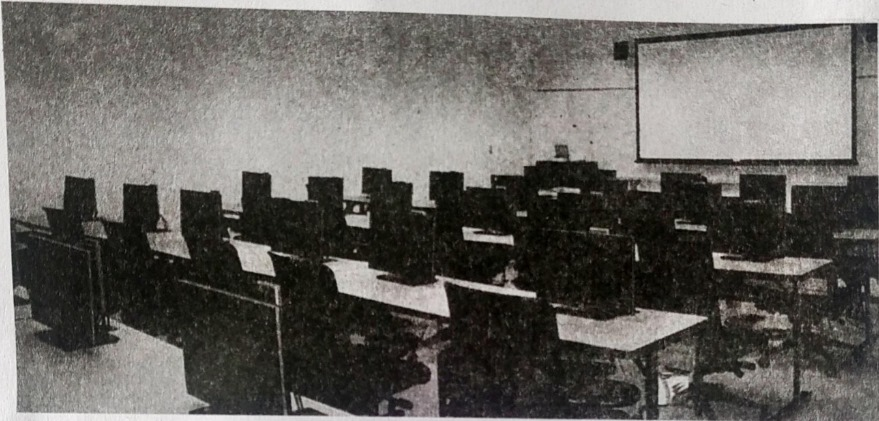
\includegraphics[width=\columnwidth]{figs/last1.jpg}
		\caption{}
		\label{fig:enter-label}
	\end{figure}

	\begin{center}
	\begin{tabular}{|c|c|c|c|c|c|}
	\hline
	\textbf{Number of computers} & 1-10 & 11-20 & 21-50 &  51-100 & 101 and more \\
	\hline
	\textbf{Number of Schools} & 250 & 200 & 290 & 180 & 80 \\
	\hline
	\end{tabular}
	\end{center}

	\text One school is chosen at random.Then:
	\begin{enumerate}
		\item  Find the probability that the school chosen at random has more than $100$ computers.
		\item
		\begin{enumerate}
			\item  Find the probability that the school chosen at random has $50$ or fewer computers.
			\item  Find the probability that the school chosen at random has no more than $20$ computers.
		\end{enumerate}
		\item  Find the probability that the school chosen at random has $10$ or less than $10$ computers.
	\end{enumerate}


\end{enumerate}
